% Source : http://tex.stackexchange.com/questions/18600/expandable-nested-boxes-with-tikz

\documentclass{article}
	\usepackage{tikz}
	\usetikzlibrary{shapes.multipart}


\begin{document}

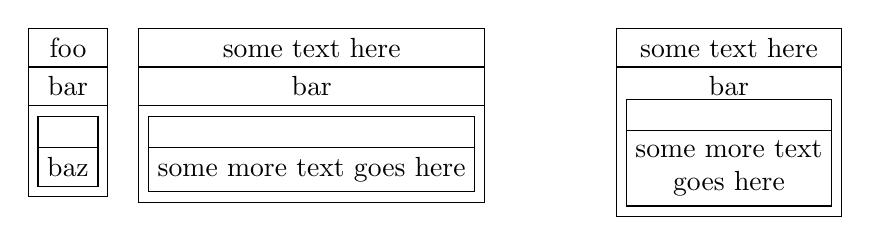
\begin{tikzpicture}[
	double/.style = {
		draw,
		anchor=text,
		rectangle split,
		rectangle split parts=2
	},
	triple/.style = {
		draw,
		anchor=text,
		rectangle split,
		rectangle split parts=3
	}
]
	\node[triple] {
		foo
			\nodepart{second}
			bar
			\nodepart{third}
				\tikz{\node[double] {\nodepart{second}baz};}
	};

	\node[triple] at (2.2,0) {
		some text here
			\nodepart{second}
			bar
			\nodepart{third}
				\tikz{\node[double] {\nodepart{second}some more text goes here};}
	};

	\node[double,align=center] at (7.5,0) {
		some text here
			\nodepart{second}
			bar \\
			\tikz{\node[double,align=center] {\nodepart{second}some more text\\ goes here};}
	};

\end{tikzpicture}

\end{document}
